\documentclass[tikz]{standalone}
\usetikzlibrary{arrows}
\usetikzlibrary{arrows.meta}

\begin{document}
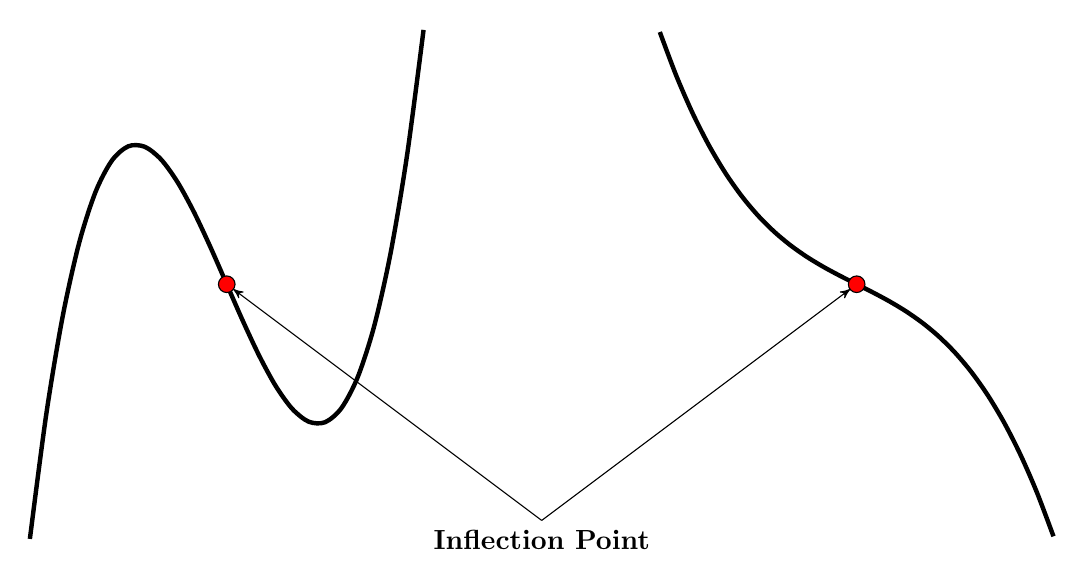
\begin{tikzpicture}[scale = 2.0]
     
% draw curve
\draw [ultra thick,smooth,variable=\x] plot [domain=-1.25:1.25] (\x,{2.3*(pow(\x,3) - \x)});
\draw [ultra thick,smooth,variable=\x,xshift=4cm] plot [domain=-1.25:1.25] (\x,{(pow(\x,3) + \x)/-2});
%\draw [ultra thick,smooth,variable=\x,yshift=-4cm] plot [domain=-1.25:1.25] (\x,{-2.3*(pow(\x,3) - \x)});
%\draw [ultra thick,smooth,variable=\x,xshift=4cm,yshift=-4cm] plot [domain=-1.25:1.25] (\x,{(pow(\x,3) + \x)/2});

% draw points
\draw [black,fill=red] (0,0) circle (1.5pt);
\draw [black,fill=red,xshift=4cm] (0,0) circle (1.5pt);
%\draw [black,fill=red,yshift=-4cm] (0,0) circle (2.0pt);
%\draw [black,fill=red,xshift=4cm,yshift=-4cm] (0,0) circle (2.0pt);

% label extrema
\draw [<-, >=stealth', shorten <=3pt] (0,0) -- (2,-1.5) node[below] {\bf Inflection Point}; 
\draw [<-, >=stealth', shorten <=3pt] (4,0) -- (2,-1.5) node[below] {}; 
%\draw [<-, >=stealth', shorten <=3pt] (0,-4) -- (2,-2.0) node[below] {}; 
%\draw [<-, >=stealth', shorten <=3pt] (4,-4) -- (2,-2.0) node[below] {}; 

\end{tikzpicture}
\end{document}
